%\documentstyle{article}  % by default 10pt
\documentclass{article}  % by default 10pt

\usepackage{graphicx}
\usepackage{amsfonts}
\usepackage{subfigure}
\usepackage{times}
\usepackage{cite}
\usepackage{subfigure}
\usepackage{amsmath}
\usepackage{amssymb}
\usepackage{url}
\usepackage{tikz}
\usepackage{verbatim}
\usepackage{array}
\usepackage{wrapfig}

%
% Page dimensions.
%
\oddsidemargin  -0.2in % 
\evensidemargin -0.2in %
\topmargin      -1.00in % (adjusted for printer bias)
\headheight      .00in  % (no headers)
\headsep         .75in  % (top margin + headers + skip)
%\footheight     12.0pt  % ??? (seems to work ok)
\footskip       75.0pt  % ??? ( "   "  )
\textheight     9.425in % (instructions: 9 1/8" min, 9 7/16" max)
\textwidth      6.7in   %
%\linespread{0.9}
%
  % Paragraph changes.
  %

  \parindent=10pt
  %\parskip=10pt
  %


  \def\@maketitle{\vbox to 2.6in{\hsize\textwidth
    \linewidth\hsize \vfil \centering
    {\large \@title \par}
    \vskip 2em
    {\normalsize
      \begin{tabular}[t]{c}\@author
	\end{tabular}\par}
      \vfil}
  }


\begin{document}

%\title{Integrated Modeling of Performance, Power and Resilience for Adaptive Parallelism}
\title{\emph{Adaptive Parallelism}: Integrated Performance, \\Power, and Resilience Modeling}


\author{Dong Li$^{\dag}$, Edgar Leon$^{\star}$, and Bronis de Supinski$^{\star}$ \\
    $^{\dag}$Oak Ridge National Laboratory and $^{\star}$Lawrence Livermore National Laboratory \\
    lid1@ornl.gov (main contact), \{leon, bronis\}@llnl.gov	\\
}

\date{}

\maketitle

\noindent {\Large \textbf{The need for integrated modeling}}\\
From embedded devices to future exascale computers, the increased
parallelism in both the number of processing units and nodes will
create unprecedented challenges to achieve the expected levels of
application performance, keep power consumption bound within a data
center's power budget or battery constraints, and maintain a system
operational in the presence of numerous failures proportional to the
size of the system. To address these challenges, modeling methods must
evolve and consider the combined effects of performance, power,
and resilience (PPR). Furthermore, modeling methods must be rapid and
accurate to dynamically evaluate the tradeoffs posed by PPR in
large-scale systems. 

% The path to exascale presents increased parallelism to reach performance targets with constrained power consumption.
% Meanwhile, efforts to reduce power and increase component counts may lead to significant increase in the number of faults,
% making system resilience a grand challenge for exascale systems.
% To address challenges of performance, power, and resilience (PPR),
% modeling methods must evolve and consider them in
% concert. Furthermore, modeling methods must be rapid and accurate,
% such that runtime can effectively enable dynamic evaluation of
% tradeoffs between PPR. 

A common practice of current modeling methods is to employ analytical
models or architectural, highly-accurate simulators. Analytical models
tend to focus on a specific dimension of performance, power, and
resilience missing their combined interdependent effects. Highly
accurate simulators, on the other hand, are not scalable. Furthermore,
the overhead imposed by many modeling tools is too high to be used at
runtime. As a result, we need more efficient and unified modeling
frameworks that would enable a runtime system to find, in real-time, a
near-optimal operating point of an application in terms of PPR. 


% The common practice of current modeling methods employs analytical models or architectural simulators to study PPR.
% The investigations of performance, power, and resilience are isolated based on individual modeling infrastructures
% and methodologies.
% Furthermore, many modeling tools and techniques are heavyweight, and cannot be easily employed at runtime.
% As a result, we do not have any efficient modeling mechanism that directs runtime management 
% and allows us to explore the optimal operating point in the 3D search space of PPR.

In this paper, we propose and infrastructure for modeling parallelism
and its combined effects on performance, power, and
resilience. Managing and optimizing parallelism dynamically is at the
core of meeting the challenging requirements of PPR imposed by future 
systems. The inherent parallelism of scientific applications varies
across execution phases~\cite{nvram_ipdps12}.  Matching the degree of
parallelism (\textit{parallel configuration}) between an application and
hardware have complicated implications on PPR~\cite{mpiopenmp_ipdps10,
  mpiopenmp_tpds13, dsn_pact08, dsn_ics06}. Our goal is to develop a
model-driven approach based on hardware resource utilization that
would allow runtime systems to determine the optimal or near-optimal
level of parallelism of a given application. 

%  We collect resource utilization information from  
% a common set of hardware components to characterize applications and
% predict PPR. 

% We study our modeling techniques in the context of runtime parallelism management for the OpenMP
% programming model.


% In this paper, we propose modeling of PPR based on an integrated %uniform 
% modeling infrastructure. 
% The infrastructure collects utilization information from 
% a common set of hardware components to characterize applications and predict PPR.
% We study our modeling techniques in the context of runtime parallelism management for the OpenMP
% programming model.
% The management and optimization of parallelism is fundamental to meet PPR requirements
% of exascale systems.
% Scientific applications typically have inherent parallelism that varies across execution phases~\cite{nvram_ipdps12}.
% Matching the degree of parallelism (named \textit{parallelism configuration} in the rest of paper) between application and hardware
% have complicated implications on PPR~\cite{mpiopenmp_ipdps10, mpiopenmp_tpds13, dsn_pact08, dsn_ics06}. 
% We aim to use a model-driven approach to decide optimal parallelism based on user-defined policies
% and enable adaptive parallelism at runtime.

%dynamic parallelism is at the core of PPR... 

%Relative order; no absoultely requirement on accuracy.
%The path to exascale presents increased parallelism with billions of concurrently-executing threads 
%at the intra-node and inter-node levels. 
%The management and optimization of parallelism is fundamental to meet performance, 
%energy-efficiency and resilience requirements
%of systems and applications at exascale.

\vspace{10pt}

\noindent {\Large \textbf{Adaptive parallelism framework}}  \\
Our proposed modeling methodology is based on two observations.
First, performance, power, and resilience have first-order or
second-order correlations with hardware components utilization.
From a performance perspective, our work reveals, for example, that
the number of accesses to the memory hierarchy and the number of
executed instructions serve as a strong indicator of performance with
various levels of parallelism~\cite{mpiopenmp_tpds13,
  mpiopenmp_ipdps10, dct_pmbs11, dct_iiswc12}. 
From a power perspective, power consumption is related to hardware
usage intensity~\cite{leon:14:characterizing,mpiopenmp_tpds13, powermodel_sigmetrics03, powermodel_micro03}.
From a resilience perspective, resilience is related to both
application execution time, $t$, and number of hardware accesses,
$hwacc$. Given hardware failure rates for specific hardware
components, a longer application execution time and a higher number of 
hardware accesses indicate that the application is more exposed to
random occurrences of hardware failures (including both hard and soft
errors). We introduce a new metric named \textit{vulnerability
  factor} (VF), which is defined as $VF = t*hwacc$, to quantify
application vulnerability. Based on this metric, resilience is also
related with hardware component utilization as it is the case for
performance and power. 

% EL: how about vf = sum over components {hwaccess(time) *
% component_failure_rate}? We don't need to explicitly state the
% formula but that vf is a function of execution time, hardware
% accesses driven by application characteristics, and component
% failure rate... 
 
Second, given a parallel region, PPR and thread-level parallelism have
a strong statistical correlation.  Hence, based on information of
hardware components utilization collected from a few samples of
parallel configurations, 
%(each of which employs a specific number of OpenMP threads),  
we can predict PPR for other parallel configurations. 
We call these representative samples \textit{seminal configurations}.

Based on the above two observations, we can construct an integrated,
PPR model in two phases: offline model training and
online model selection. During the first phase, we use a machine
learning-based approach to determine the hardware components
utilization information that is most correlated with PPR.  
Hardware utilization should be measurable with lightweight hardware
counters. Also, seminal configurations are chosen empirically.
Empirical observations reveal that PPR data with different levels
of parallelism can be clustered into different groups. The parallel configuration
which is the \emph{closest} to the center of each group is chosen as a 
seminal configuration. 
% EL: we need to explain what we mean by "closest"
During offline training, we build a series of PPR models to
capture diverse hardware features and application
characteristics. Using a diverse set of applications and benchmarks
during training is key to produce accurate models. 
During online model selection, we use a few sample iterations of
parallel regions to execute with seminal configurations and collect
hardware components utilization information, based on which we
identify the model that should be employed to predict PPR. 

Based on the above modeling methodology, we can accurately predict PPR
at runtime for any untested parallelism configuration with low
overhead. This is possible since the model is built offline using
a diverse set of application characteristics. Using
the resulting models, a runtime system can be 
guided by high-level policies that indicates the desired levels of
performance, power, and resilience. For example, minimizing the
vulnerability factor at a marginal performance and power cost; and
achieving the best performance and resilience within a power
cap. Figure~\ref{fig:general_framework} provides an overview of our 
framework's model construction and deployment.

% Built on top of the models,
% runtime chooses the best parallelism for each OpenMP parallel region based 
% on high-level user-defined policies, for example, minimizing VF without performance and power
% loss, or minimizing the multiplication of time, power, and VF to achieve
% an optimal tradeoff of PPR, or achieving the best performance and
% resilience within a power cap.
Our previous investigations show that this methodology can
predict performance and power with high accuracy on many-core
platforms. These results are encouraging and we plan to integrate our
proposed resiliency model into this framework. Looking forward, future
milestones include the creation of models for emerging heterogenous
memory architectures (multiple levels of memory to provide future
bandwidth and capacity requirements), analyzing the effects of data
layout and memory parallelism on PPR, and developing new models for
heterogenous computing platforms. We plan on leveraging our expertise
on OpenMP as a vehicle to implement our proposed infrastructure. 

% We have established the model infrastructure to predict performance and power on many-core platforms.
% We plan to extend the modeling methodology to better capture effects of
% data layout and memory-level parallelism on PPR.
% We also plan to extend the models to support PPR prediction 
% and parallelism scheduling on
% heteroegenous platforms. 
%to be a new layer between OpenMP directives,

\begin{wrapfigure}{r}{0.4\textwidth}
\begin{center}
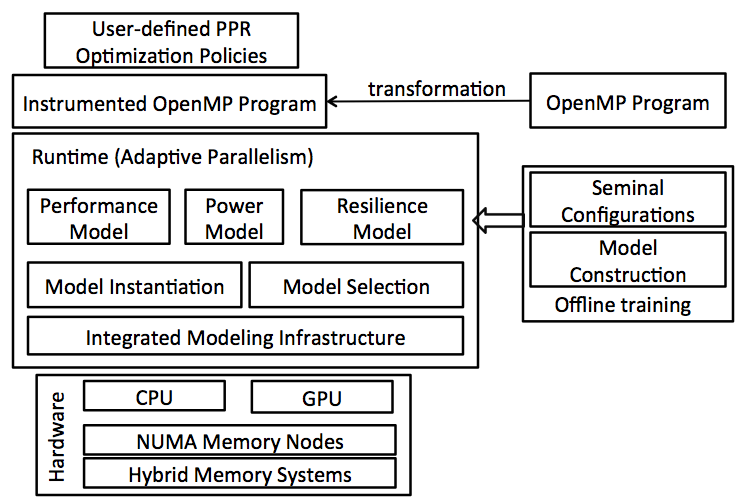
\includegraphics[width=0.39\textwidth]{figures/general_framework.png}
\end{center}
\caption{The general framework for adaptive parallelism with integrated PPR modeling}
\label{fig:general_framework}
\end{wrapfigure}

\vspace{10pt}

\noindent {\Large \textbf{Related work}}   \\
Performance, power, and resilience modeling and simulation have been
studied before, but mostly in isolation. Some of the related work employ
analytical or empirical models to achieve joint optimization of power
and performance. For example, Green Queue~\cite{sdscpower_hppac12,
  sdscpower_ccpe12, sdscpower_cgc12},  Adagio~\cite{rountree_sc07,
  rountree_ics09}, and Workload
Consolidation~\cite{taskconsolidation_ipdps10,   gpusolidation_srmpds11}. 
Other work use detailed hardware analysis for hardware-oriented resilience modeling. 
For example, Mukherjee et al.~\cite{avf_micro03} define an
architectural vulnerability factor (AVF) as the probability that a
fault in a particular structure will result an error. Biswas et
al.~\cite{avf_isca05} show how to compute the AVF of address-based
processor structures based on a detailed analysis of architecturally
correct execution. Sridharan and Kaeli~\cite{pvf_selse10, pvf_hpca09}
introduce a new metric to capture the architecture-level fault masking
inherent in a program. In addition, fault injection has been
widely used to understand application vulnerability in  
~\cite{li:2012:classifying, multigrid_ics12, fj_asplos12, fj_dns12,
  lanl_fi_europar11}.

\vspace{10pt}

%Challenges addressed: Which modeling and/or simulation challenges
%does this approach address? 
\noindent {\Large \textbf{Evaluation of proposed methodology}}   \\
\textbf{Challenges}. 
Future systems demand modeling and simulation capabilities to help us
understand the complex and combined interactions between performance,
power, and resilience. Furthermore, modeling and simulation techniques
should provide rapid and dynamic evaluation of tradeoffs between
PPR. Our proposed modeling infrastructure is designed to provide a
light-weight and accurate prediction of PPR based on adaptive
parallelism. It can be used by runtime systems to manage system
resources for a specific set of objectives based on thread-level and
memory-level parallelism.  

%extremely
%valuable for runtime management of system resource (e.g., thread-level parallelism and  
%memory-level parallelism in our case).
%The proposed approach addresses resilience and power challenges for future exascale systems as

%Maturity: What are the indicators that this approach will address the
%identified challenges? 
\noindent\textbf{Maturity}. 
Our previous investigations show that our
proposed methodology can provide accurate and light-weight modeling 
of performance and power for OpenMP parallel regions on several
multi-core architectures. We have successfully applied
machine-learning techniques to this area to address the challenges
associated with an extremely large space of optimizations. We believe
that this infrastructure provides a strong basis for integrating
modeling of different objective functions. Adding modeling
capabilities for resilience and reliability along with processor and
memory heterogeneity will undoubtedly present significant challenges. 

% Performance, power and resilience modeling and simulation have been separatrely considered in the
% existing work (see related work).
% Also, we have established preliminary capabilities to model performance and power for OpenMP parallel 
% regions with various parallel configurations. Our modeling infrastructure brings ignorable 
% performance overhead while providing great energy saving for DOE applications with 
% the hybrid MPI/OpenMP programming model.
% However, our current modeling infrastructure is only a start and
% requires significant new work to improve modeling infrastructure
% especially for resilience modeling and heterogeneous platform. 
%The proposed idea builds on successful research, including the DOE funded Blackcomb 

%Uniqueness: To what extent is the proposed approach unique? Could it
%be addressed by other research programs? 
\noindent\textbf{Uniqueness}.
A key feature of our modeling methodology is our focus on
parallelism as we believe is at the core of managing the tradeoffs
between power, performance, and resilience. In addition, we propose
using machine-learning techniques to create multi-dimensional models
of performance, power, and resilience. The goal of our modeling
infrastructure is to guide a runtime system to determine the
\emph{right} level of concurrency to achieve desired optimization
objectives. 

% Our modeling methodology is tightly coupled with the OpenMP programming model,
% and aims to reveal PPR difference between different parallelism configurations.
% Unlike prior work that focuses on accurate prediction, our work
% focuses on coarse-grained PPR indicator to guide runtime management. 

%Novelty: How is this approach different from existing solutions?
\noindent\textbf{Novelty}. 
Our modeling methodology reveals statistical correlation
between measurable hardware events, application characteristics, and 
PPR. The unique set of features and opportunities provided by our models
provide fast exploration of PPR to achieve multi-dimensional optimization.     

%Applicability: To what extent will the proposed approach, if
%successful, be applicable to other areas? 
\noindent\textbf{Applicability}. 
The proposed PPR models have been deployed in an OpenMP runtime to
optimize performance and energy efficiency by using adaptive
parallelism. We believe that this approach can be successfully applied
to other areas such as modeling of emerging memory systems. 

% The proposed models work
% as a critical step to implement adaptive parallelism, 
% and provide a new approach for massive parallelism management.

%Effort: How much effort is needed to effectively explore this approach?
\noindent\textbf{Effort}. 
Key milestones include developing models
of resilience and memory-level parallelism and investigating their
interactions with other 
objectives such as power and performance. In addition, we need to
investigate the accuracy and overhead of our modeling methodology on a
variety of hardware  resources including homogenous and heterogenous
processor 
architectures, and emerging heterogeneous memory architectures
(multi-level memories). 

% We need to add new features into the current modeling infrastructure,
% including resilience modeling and memory-level parallelism modeling,
% and interoperating with other ModSim tools.
% To provide a broad coverage of system properties and resources, we need
% a significant effort contributing to an agile and integrated modeling
% of PPR.

\bibliography{li}
\bibliographystyle{plain}

\end{document}
